\section{Switch Based Models}
The switching state-space Model (SSSM)~\citep{ghahramani2000variational}, or switching linear dynamical system (SLDS)~\citep{fox2009nonparametric}, captures nonlinear dynamical phenomena by allowing discrete points in time where a system switches among conditionally linear dynamical modes. Our primary reason for exploring this model is to perform inference over the assignment of data to specific linear dynamical modes (or regimes), thereby characterizing periods that exhibit dynamics controlled by the regimes. The ease of interpretability of the conditionally linear regimes is an attractive merit of this model, yet the presence of the discrete switch points allows the model to capture a wide variety of non-linear dynamics.

The SSSM has been used for prediction tasks~\citep{fox2007hierarchical,li2003survey} but also for inference tasks~\citep{fox2009nonparametric,jonsen2007identifying,pavlovic2001learning} where the primary goal was to discover latent structure in time series data. \citet{oh2008learning} use the term `learning' to describe the segmentation of the motion of honey bees into different behavioral regimes. They describe the identification of the parameters that characterize the motion within a regime as `quantification'. Similarly, we aim to (1) `learn' the \textit{periods} that define salient regimes in the CW simulation and (2) `quantify' these regimes for the purpose of generating a useful description of the system dynamics.

This work is broadly related to the field of mining information from time series data~\citep{esling2012time,horst2004data}. In contrast to the switching systems that we discuss, other approaches have aimed to cluster short segments from time series data to identify certain patterns that might arise in a database~\citep{vlachos2003wavelet,tanaka2005discovery,patel2002mining}. This involves windowing a time series and defining wavelets, motifs~\citep{patel2002mining} or segments that are commonly found throughout the database. \cite{preston2009event} propose an approach to define and mine for events in a time series database. These previous approaches are concerned with finding small sections or events that might be of relevance within the larger time series. We rather focus on decomposing the \textbf{entire} time series into periods that are coherent to a human observer.

\citet{ghahramani2000variational} introduce and give a detailed presentation of the SSSM. \citet{pavlovic2001learning} and \citet{giordani2007unified} use switching models to capture non-linear behavior in a time series, applied to model human motion and econometrics respectively. SSSMs have also been applied in object tracking domains where it is necessary to predict the trajectory of multiple objects~\citep{fox2007hierarchical}. \citet{whiteley2010efficient} introduce a sequential Monte Carlo algorithm for inference over SSSMs using discrete particle filters. We present a new avenue of study in which SSSMs are used to describe complex time series in a way that can be easily interpreted by people and we propose an algorithm to perform posterior inference over the latent variables in this model.

Before describing the SSSM in Section~\ref{sec:switching_state_space_models}, we first provide a brief introduction to the linear state-space model for \textit{continuous} time series data and the hidden Markov model for \textit{discrete} time series data. The SSSM couples these two models and thus this background work is a necessary step towards constructing the SSSM.


\subsection{Background}
\subsubsection{State Space Models and Hidden Markov Models}\label{sec:state_space_and_hidden_markov_models}
Hidden Markov models (HMM) and state-space models (SSM) define a joint probability density over a sequential collection of hidden state ($\mathbf{X}$) and observed ($\mathbf{y}$) random vectors~\citep{ghahramani2001introduction,shumway2000time}. The HMM refers to the case when the states and observations have discrete values. For example at a time step $t$ the hidden state $\mathbf{X_t}$ is represented by a categorical variable that can take one of $M$ possible discrete values, where a value indexes a state. The associated observations $\mathbf{y_t}$ are discrete symbols where the observation probabilities $P(\mathbf{y_t} \mid \mathbf{X_t})$ can be fully specified by an $M \times K$ observation matrix, with $K$ being the number of possible observation states. Given the hidden state at time $t$ in an HMM, the associated observation is independent from all other observations. Moreover, the hidden states obey the Markov independence property: state $\mathbf{X_{t}}$ is conditionally independent from the previous states ($\mathbf{X_{k}}$ for $k \in 1,2, \hdots, t-2$) and future states ($\mathbf{X_{k}}$ for $k \in t+2, \hdots, T$) given the value of state $\mathbf{X_{t-1}}$ and $\mathbf{X_{t+1}}$ respectively. The joint probability for the sequence of states and observations can be factored as\footnote{Here we use the notation $X_{1:t}$ to refer to all states $X_k, k \in [1,2,\hdots,t]$}:

\begin{equation}\label{eq:joint_prob_ssm}
  P(\mathbf{X_{1:T}}, \mathbf{y_{1:T}}) = P(\mathbf{X_1})P(\mathbf{y_1} \mid \mathbf{X_1}) \prod\limits_{t=2}^{T} P(\mathbf{X_t} \mid \mathbf{X_{t-1}} ) P( \mathbf{y_t} \mid \mathbf{X_{t}} )
\end{equation}

When the model is changed to allow for real-valued state and observation vectors, it is termed a state-space model. The simplest and most commonly used models that follow this structure assume that the transition and output functions are linear and time invariant and the distributions of the state and observation variables follow multivariate Gaussian distributions~\citep{ghahramani2000variational}. The linear Gaussian SSM is defined by the tuple $(A, C, Q, R)$ in:
\begin{equation}\label{eq:hmm_first_order}
  \begin{split}
      \mathbf{X_t} &= A\mathbf{X_{t-1}} + w_t \\
      \mathbf{y_t} &= C\mathbf{X_t} + v_t
  \end{split}
\end{equation}
where $A$ is the state transition matrix, $w_t \sim \mathcal{N}(0,Q)$ is the state transition noise, $C$ is the output matrix and $v_t \sim \mathcal{N}(0,R)$ is the observation noise.

The problem of inference or state estimation for a SSM with known parameters consists of estimating the posterior probabilities of the hidden variables given a sequence of observed values. This inference problem can be broken into \textit{filtering}, \textit{smoothing} and \textit{prediction}~\citep{shumway2000time}. The goal of filtering is to use all the data up to time $t$ to calculate the probability of the hidden state $X_t$. Smoothing, aims to use all of the data available from time $1 \hdots T$ (with $T > t$) to calculate the probability of $X_t$. Lastly, prediction is calculating the probability of the future states $X_{t+1}$ given all the data from time $1 \hdots t$. A minor terminology note is that when we perform filtering and smoothing in the context of linear Gaussian state space models, the algorithms are termed Kalman filtering and smoothing respectively.

\subsubsection{Forward Algorithm}
The forward algorithm, also termed filtering, aims to calculate the probability that a certain state $X_t$ adopts a specific value using only data that is available up to that point in time ($y_{1:t}$). The joint probability of the latent state and the previous data is:

\begin{equation}\label{eq:fwd_filter}
  \begin{split}
    P(X_t, y_{1:t}) &= \sum_{X_{t-1}} P(X_t, X_{t-1}, y_{1:t}) \\&= P(y_{t} \mid X_t) \sum_{X_{t-1}} P(X_t \mid X_{t-1})P(X_{t-1}, y_{1:t-1})
  \end{split}
\end{equation}

We have applied the Markov independence property where: 
\begin{equation}
	\begin{split}
	y_{t}~\mid~X_t &~\indep~y_{1:t-1},~X_{1:t-1} \\
    X_{t}~\mid~X_{t-1} &~\indep~y_{1:t-1},~X_{1:t-2}
    \end{split}
\end{equation}

Note that the joint probability $P(X_{t-1}, y_{1:t-1})$ can be expressed in the same form as equation~\ref{eq:fwd_filter} but dependent on $P(X_{t-2}, y_{1:t-2})$. This defines an efficient recursive routine for calculating the probabilities for all states up to time $t$ using the past data $y_{1:t}$. Note that $P(y_{t} \mid X_t)$ and $P(X_t \mid X_{t-1})$ are given by the transition and emission probabilities (or the emission likelihood in the SSM) and this recursion can be efficiently implemented using a dynamic programming implementation.

\subsubsection{Backward Algorithm}
It is not always the case that we need to analyze time series data in a streaming fashion (i.e. where data arrive in real time and we only use past and present data to make state estimation inference). When the data are available in an off-line setting, it is advantageous to use \textit{future} values to help calculate the probability of the state at time $t$. The backward algorithm, also termed smoothing, achieves this by calculating the probability of $X_t$ by using all available data $y_{1:T}$, with $t < T$. The backward recursion depends on the value of the forwards filter and a new term that can be factored similarly to equation~\ref{eq:fwd_filter}.

\begin{equation}\label{eq:bkwd_filter1}
  \begin{split}
    P(X_t, y_{1:T}) &= P(y_{1:t}, y_{t+1:T}, X_t) =  P(y_{1:t}, y_{t+1:T} \mid X_t)P(X_t)\\ &= P(y_{t+1:T} \mid X_t)[P(y_{1:t} \mid X_t)P(X_t)]
  \end{split}
\end{equation}

$P(y_{t+1:T} \mid X_t)$ corresponds to calculating the probability of observing the future data given the current state (called backward values). $P(y_{1:t} \mid X_t)P(X_t) = P(y_{1:t}, X_t)$ is the probability from the forward algorithm in equation~\ref{eq:fwd_filter}. We are now able to factor the backward term, again using the Markov independence property:

\begin{equation}\label{eq:bkwd_filter2}
  \begin{split}
    P(y_{t+1:T} \mid X_t) &= \sum_{X_{t+1}} P(y_{t+1:T}, X_{t+1} \mid X_t) \\&= \sum_{X_{t+1}} P(y_{t+1:T} \mid X_{t+1})P(X_{t+1} | X_{t})
  \end{split}
\end{equation}

We can calculate the term $P(y_{t:T} \mid X_{t})$ in terms of $P(y_{t+1:T} \mid X_{t+1})$ thereby defining the set of backward recursions that are needed to calculate fully the joint probability in equation~\ref{eq:bkwd_filter1}. This recursion is given by:
\begin{equation}\label{eq:bkwd_filter3}
  \begin{split}
    P(y_{t:T} \mid X_t) &= \sum_{X_{t+1}} P(y_t, y_{t+1:T}, X_{t+1} \mid X_t) \\&= P(y_t \mid X_t) \sum_{X_{t+1}} P( y_{t+1:T} \mid X_{t+1} ) P( X_{t+1} \mid X_t )
  \end{split}
\end{equation}

One would therefore start the backward recursion from time $T$ to calculate successively the joint probabilities of the states $X_{t:T}$. From equation~\ref{eq:bkwd_filter1}, it can be seen that the forward and backward recursions are both used to calculate the probability of $X_{t}$ given all of the data $y_{1:T}$. In practice, the forward algorithm is run for one pass of the data from $t=1$ to $t=T$ and then the backward algorithm is run from $t=T$ to $t=1$. Note that we have referred to the HMM in the above equations (the marginalizing steps are summations) but appropriate adjustments (to integrals) will present the SSM filtering and smoothing recursions.

\subsubsection{Viterbi Algorithm}\label{sec:viterbi_algorithm}
The Viterbi algorithm~\citep{forney1973viterbi} for HMMs recursively finds the most probable path of states that generated the observed data~\citep{nasrabadi2007pattern}. We first define the partial probability $\pi_{t,i}$ to be the probability of the best path for states $X_{1:t}$ that leads to state $X_t = i$. Intuitively, the best path leading to state $X_t = i$ at time step $t$ must include the best path to $X_{t-1}$ (assuming the same ending state $i$). We can therefore expect a recursive structure to an algorithm that decodes the best state sequences. In the following, we denote $X_i$ as all possible terminating states that can be adopted at the time step $t$.
\begin{equation}\label{eq:viterbi}
  \pi_{t,i} = \max\limits_{\forall X_i} \left\{ \pi_{t-1,j} P(y_t \mid X_i)P(X_i \mid X_{t-1}) \right\}
\end{equation}

The algorithm uses the maximum probability from the previous state along with the observation probabilities for decoding the most likely present state. These can be stored in a table and the most likely state sequence is the maximum at each time step.



\subsection{Switching State Space Models}\label{sec:switching_state_space_models}
A SSSM includes $M$ latent continuous state-space models and a discrete switching variable. Each of the models, referred to as a regime, has its own dynamics. At each point in time, the switching variable selects one of the individual state-space models to generate an observation vector.

The SSSM model is formalized as:
\begin{equation}
  \begin{split}
      \mathbf{X^{(m)}_t} &= \Phi^{(m)}\mathbf{X}^{(m)}_{t-1} + w^{(m)}_t \\
      \mathbf{Y_t} &= S_t A^{(m)}\mathbf{X}^{(m)}_t + v_t
  \end{split}\label{eq:switching_state_space}
\end{equation}

Here, $X_t^{(m)}$ denotes the latent continuous valued state for process $m$ at time $t$. $S_t$ is a discrete valued switching variable that selects the $m^{th}$ regime such that regime $m$ at time $t$ is active. The real-valued state $X_t^{(m)}$ and the parameters associated with the $m^{th}$ regime produce the real-valued observation vector $Y_t$. The states' evolution over time depends on the regime dependent transition matrix $\Phi^{(m)}$ and the regime dependent noise $w_t^{(m)}$. When the states and observations are assumed to follow Gaussian distributions, each regime can be viewed as a linear Gaussian SSM as discussed in section~\ref{sec:state_space_and_hidden_markov_models}.

Figure \ref{fig:switching_ssm} presents a graphical representation of a SSSM. Edges between nodes represent conditional dependencies, gray nodes are observed variables and white nodes are latent variables. Not shown in the figure are the regime dependent transition noise $w_t^{(m)}$ and the observation noise $v_t$ which have the same interpretation as the noise models in the SSM. $A^{(m)}$ is the output matrix in the state space formulation, which can be regime dependent but for the applications that follow, it is taken to be the identity matrix.

\begin{figure}
  \centering
  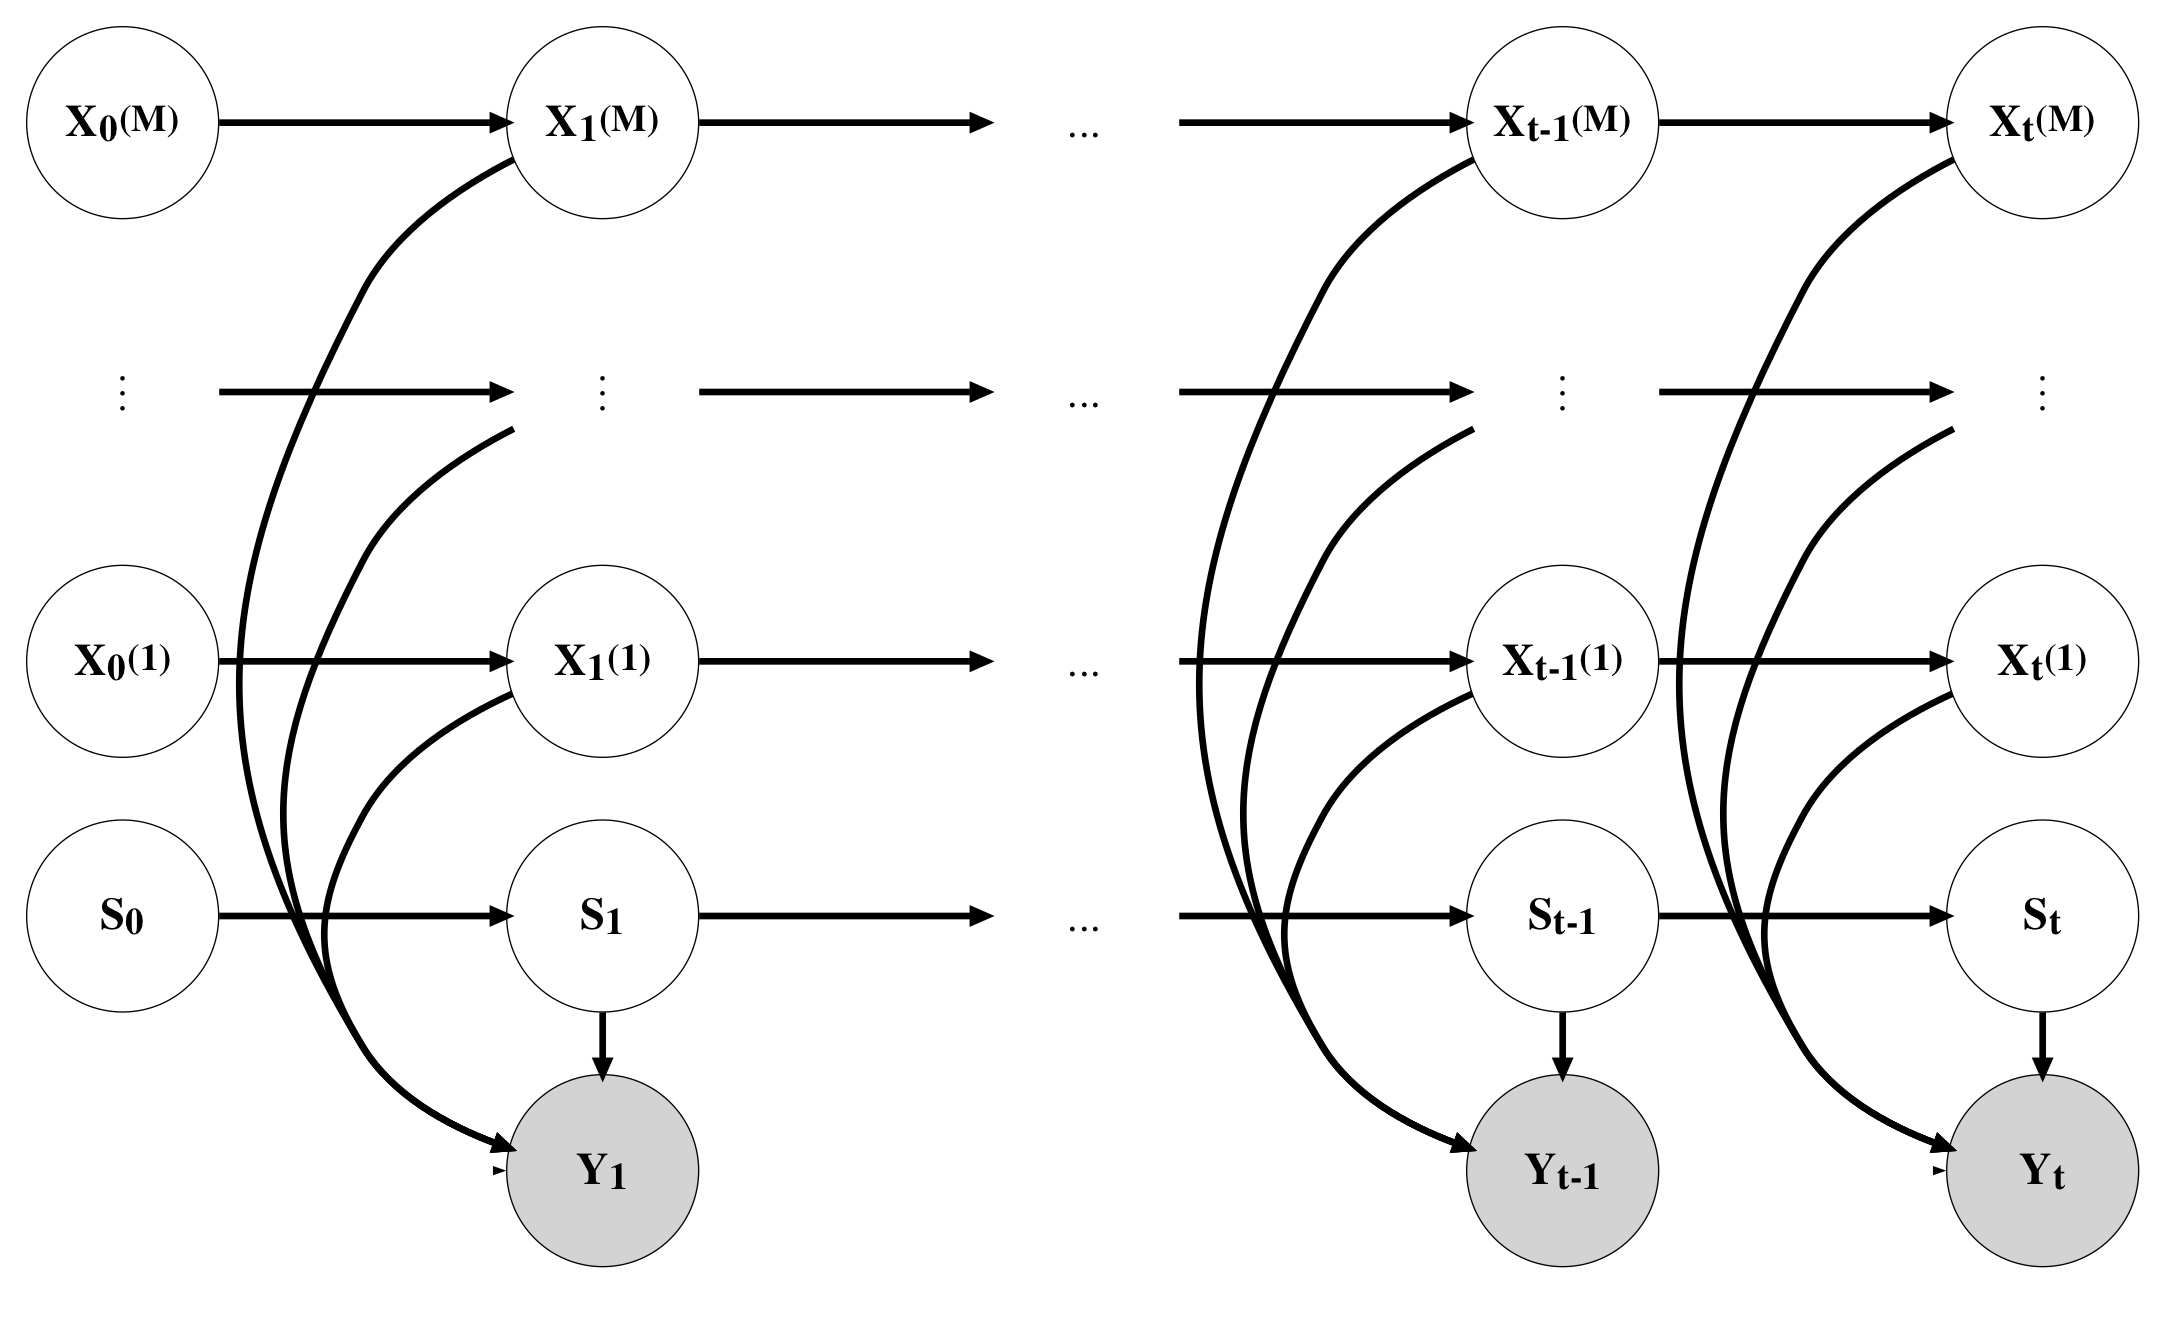
\includegraphics[width=12cm]{switching_ssm.png}
  \caption{Graphical model for the switching-state space model. A latent discrete switching variable ($S_t$) selects an active, real-valued state space model ($X^{(m)}_t$). The observation vector ($Y_t$)  depends on the active regime at time $t$.}
  \label{fig:switching_ssm}
\end{figure}

\subsection{Interpretability of the SSSM}\label{sec:interpretability_of_ssm}
We illustrate the SSSM interpretability by presenting an example of how it can describe the effects of students' interactions in CW. $Y_t$ represents the observed water level in the different areas of the simulation at time $t$. $X_t^{(m)}$ describes the expected levels of water under regime $m$ at time $t$. $\Phi^{(m)}$ controls the water flow in the simulation according to the transitions in regime $m$. $S_t$ selects which of the regimes to use to describe the water levels $Y_t$.

A single regime is insufficient for modeling the effects of students' interactions with CW. This is because students' actions have complex effects on the system dynamics. For example when students choose to direct water to the Desert and Plains and plant many trees in the Desert, the system dynamics are entirely different to the case when water is directed towards the Jungle and the Desert and the Plains are left to dry. We therefore need to define multiple regimes, where each regime describes a series of events that can be (stochastically) explained by the regime dynamics. A regime is active for a duration of time in CW. This duration is called a period. In our example, in one period, water is mainly flowing to the Plains and to the Desert. In the next period, students move the logs to re-route water flow to the Jungle (potentially because plant life is dying). The students may also release water from the Reservoir to direct that to the Desert. These dynamics will be captured by the second period's regime parameters. The output of the model is a number of regimes (that are active for the corresponding periods) that together capture the system dynamics, but individually can be easily interpreted.

Note that we have described a system where the direct observation of the underlying process is available. This is termed a vector autoregressive model (VAR) with switching~\citep{fox2009nonparametric, shumway2000time,kim1994dynamic}. An order $r$ VAR process with observations $\mathbf{y_t}$ is defined by:
\begin{equation}\label{eq:var}
  \mathbf{y_t} = \sum\limits_{i=1}^{r} A^{(m)}y_{t-i} + w^{(m)}_t \hspace{20pt} w^{(m)}_t \sim \mathcal{N}(0, Q^{(m)})
\end{equation}

Equation~\ref{eq:var} shows that the observations at time $t$ depend linearly on the previous $r$ observation vectors. In CW, we use a $VAR(1)$ process. Since the SSSM generalizes the switching $VAR$ process, we refer to the SSSM throughout this study but recognize that the models also apply to the VAR specific case. Any $VAR(r)$ process can be written in a SSM format as follows:

\begin{equation}\label{eq:ssm_rep_of_var_state}
  \mathbf{X_t} =
  \begin{bmatrix}
      A_{1}       & A_{2} &  \dots & A_{r} \\
      I           & 0     &  \dots & 0 \\
      \vdots      & \ddots&  \vdots& \vdots \\
      0           & \hdots&   I    & 0
    \end{bmatrix} \mathbf{X_{t-1}} +
  \begin{bmatrix}
    I \\
    0 \\
    \vdots \\
    0
  \end{bmatrix} w^{(m)}_t
\end{equation}

\begin{equation}\label{eq:ssm_rep_of_var_output}
  \mathbf{y_t} = \begin{bmatrix} I & 0 & \hdots & 0 \end{bmatrix} \mathbf{X_t}
\end{equation}

It is worth highlighting that for the SSSM in general, and indeed for the inference that we target in CW, the model is highly under-specified. The points in time that define the changes between regimes are unknown, the duration of the periods are unknown and the regime specific parameters are unknown. Moreover, the number of regimes is unknown. The goal of Section~\ref{sec:posterior_inference_sssm} is to introduce an efficient unsupervised algorithm for performing inference over these unknown variables. For this implementation, we define a reasonable number of regimes $M$ but in Section~\ref{sec:non-parameteric} we discuss the related work in Bayesian non-parametrics which allow us to remain agnostic about the number of regimes that are present.


\section{Inference for Switching State Space Models}\label{sec:inference_for_sssm}
We aim to perform inference over the latent states $X_t^{(m)}$, the regime parameters $\Phi^{(m)}$, and latent switching variable $S_t$ in the SSSM defined in E
equation~\ref{eq:switching_state_space}. Computing posterior distributions for SSSMs is computationally intractable~\citep{murphy2002dynamic, kim1994dynamic}. To illustrate, in Figure~\ref{fig:switching_ssm} note that the graph consists of $M$ state space models that are marginally independent. These models become conditionally dependent when $Y_t$ is observed (as is the case in this graph). The result is that $X_t^{(m)}$ is conditionally dependent on the value of all of the other latent states and switching variables for times $1$~through~$T$ and regimes $1$~through~$M$~\citep{murphy2002dynamic,ghahramani2000variational}.

Due to the intractability, previous approaches use approximation methods such as variational inference~\citep{ghahramani2000variational} or a `merging of Gaussians'~\citep{kim1999state,murphy2002dynamic} to address the inference problem. Variational inference approximations transform the intractable Bayesian expectation problem into an optimization problem by minimizing the Kullback-Leibler divergence between a simpler family of approximating distributions and the unknown, intractable posterior~\citep{attias2000variational,saul1996exploiting,saul1996mean,blei2003latent}. The merging of Gaussians uses a single Gaussian to approximate the mixture of $M$ Gaussians at each time step. While these methods have seen success in previous examples, they cannot be applied to our domain. This is because they allow the system to move back and forth between regimes, resulting in frequent regime changes that can hinder the interpretability of the model. This work takes a different approach by imposing structure on the model to address both inference and interpretability challenges. Another avenue for inference is the sticky hierarchical Dirichlet process hidden Markov model (sticky HDP-HMM)~\citep{fox2009nonparametric,fox2007hierarchical}, an extension of the hierarchical Dirichlet process (HDP)~\citep{teh2005sharing}, that relaxes the within-cluster exchangeability assumption of the HDP. We discuss this model in further detail in Section~\ref{sec:non-parameteric} and present it as a promising avenue for future work.

To perform inference over the regime parameters and the switch assignments, we make two assumptions, which arise from the need to create human interpretable descriptions of the complex system behavior. \textbf{Assumption 1:} the system advances through a series of regimes, each regime is active for a period, and then switches to an entirely new regime, one that has not been used before. \textbf{Assumption 2:} the regime remains active for the maximum possible time for which it can be used to describe the period.

Without making these assumptions there are $M$ possible assignments of regimes for each time step, making a total of $M^T$ combinations of possible assignments, which is exponential in the number of time steps. Moreover, in the worst case, the number of possible periods is bounded by $T$ with a switch at every time step. In contrast, under our assumptions, there are only two possible assignments of regimes for each time step (i.e., the choice is to stay in the current regime or to progress to the next regime), making for a total of $2^M$ combinations of possible assignments, where $M$ is constant.  The number of possible periods under this methodology is bounded by $M$.
% We further hypothesize that the forced reduction in complexity of the fitted model would significantly simplify the interpretability of the model for a human.

\subsection{Approximate Maximum Likelihood Estimation for Switching State Space Models}\label{sec:gaussian_merging}

\cite{shumway1991dynamic} assume known regime parameters and use the state space specific observation probabilities to perform inference over the switching variables in the SSSM (using the Viterbi algorithm presented in \ref{sec:viterbi_algorithm}). Their implementation is extended by \cite{kim1994dynamic, kim1999state} and \cite{bar1993estimation} to handle the case where the regime parameters are unknown. The maximum likelihood estimate (MLE) presented by these authors employs a `Gaussian merging' assumption~\citep{ghahramani2000variational} to make the inference tractable. \cite{kim1994dynamic} presents a basic filtering and smoothing algorithm for the SSSM, combined with a MLE of the unknown regime parameters.

In the standard state space filtering formulation, we wish to calculate the expected value of the latent states $X_t$, given the observations $y_{1:t}$. This corresponds to calculating:
\begin{equation}\label{eq:kim_ssm_expected_val}
  X_{t \mid t} = E[X_t \mid y_{1:t}]
\end{equation}
Following state space notation for the expectation, $X_{t \mid t}$ refers to the expected value of the latent state at time $t$ given the previous observations. Similarly, $P_{t \mid t}$ refers to the covariance of the estimate for $X_{t \mid t}$ conditioned on the data $y_{1:t}$:
\begin{equation}\label{eq:kim_ssm_covariance}
  P_{t \mid t} = E[(X_t - X_{t \mid t})(X_t - X_{t \mid t})' \mid y_{1:t}]
\end{equation}
With the introduction of the switching variable $S_t$, we require the expectation $X_{t \mid t}^{(i,j)}$ which is the expected value for $X_t$, conditioned on the past data $y_{1:t}$ and the value of $S_t = j$ and $S_{t-1} = i$. The expected values for the state and the covariances associated with these estimators are:

\begin{equation}\label{eq:kim_sssm_expected_val}
	\begin{split}
  X_{t \mid t}^{(i,j)} &= E[X_t \mid y_{1:t}, S_{t-1} = i, S_t = j] \\
  P_{t \mid t}^{(i,j)} &= E[(X_t - X_{t \mid t})(X_t - X_{t \mid t})' \mid y_{1:t}, S_{t-1} = i, S_t = j]
  	\end{split}
\end{equation}

In computing the Viterbi algorithm, we would require the expectations and covariances in equations~\ref{eq:kim_sssm_expected_val} for every possible value for $i$ and $j$. If there are $M$ regimes in the model, this results in $M^2$ terms that are calculated at every time step. The resulting Kalman filter experiences a growth of terms that is exponential in $T$, a problem that is also encountered in Section~\ref{sec:posterior_inference_sssm}. \cite{kim1994dynamic} proposes an algorithm for reducing the $(M \times M)$ posteriors for $X_{t \mid t}^{(i,j)}$ into just $M$ posteriors by merging the Kalman filter to a single posterior at each time step.

The approximation that \cite{kim1994dynamic} employs is given by:
\begin{equation}\label{eq:collapsed_likelihood}
  X_{t \mid t}^{(j)} = \frac{\sum\limits_{i=1}^{M} P[S_{t-1}=i, S_t=j \mid y_{1:t}]X_{t \mid t}^{(i,j)}}{P[S_t = j \mid y_{1:t}]}
\end{equation}
\cite{ghahramani2000variational} call this the `Gaussian merging' approach because in equation~\ref{eq:collapsed_likelihood}, $X_{t \mid t}^{(j)}$ represents the re-normalized mixture of Gaussians in the numerator. $X_{t \mid t}^{(j)}$ represents the $E[X_t \mid S_t = j, y_{1:t}]$ with the $S_t = i$ dependency marginalized out. The covariance of this estimator $P_{t \mid t}^{(j)}$ is calculated in a similar fashion and can also be interpreted as the posterior from a weighted mixture of normals\footnote{See the derivation in \cite{kim1994dynamic} for further details.}.

Finally, we can use numerical optimization to perform parameter estimation. The Gaussian merging is used to construct a forward filter to approximate the likelihood of the regime parameters and the associated switches. This likelihood is maximized to present an approximate MLE for the parameters. It is worth noting that the optimization is highly susceptible to local maxima due to the tightly coupled nature of the regime parameters and the locations of the switch points. Thus, the numerical optimization might terminate early at these local optima leading to incorrect inferences. This is seen in Section~\ref{sec:experiment1-empirical-validation}.

\subsection{Background on Inference for Probabilistic Models}

\subsubsection{Introduction to Bayesian Inference}

Bayesian models lend themselves to domains where the interpretability of the model is of importance~\citep{gelman2014bayesian}. The model structure that is imposed on a domain is considered part of the prior knowledge and as such, inference about the latent variables has a strong interpretability within the defined model's structure. Bayesian statistics is derived from Bayes rule:

\begin{equation}\label{eq:bayes_rule}
	P(\theta \mid X) = \frac{P(X \mid \theta)P(\theta)}{\int P(X \mid \theta)P(\theta) d\theta}
\end{equation}

The denominator in equation~\ref{eq:bayes_rule} represents the normalizing constant that is not dependent on the parameter vector $\theta$. This integral is often intractable and thus evaluation of the posterior $P(\theta \mid X)$ becomes a challenging objective. Conjugate structure in certain problems allows for the direct computation of an analytical solution for the posterior distribution. This structure is often not available, or conjugacy imposes undesirable restrictions given the problem setting. Thus other means for \textit{approximating} the posterior distribution are required when performing inference in Bayesian models. Variational inference~\citep{attias2000variational,saul1996exploiting,saul1996mean,blei2003latent} is an approach that is commonly used to approximate the posterior distribution. Variational inference can give misleading results when dealing with highly correlated and co-dependent data, such as data present in time series models~\citep{turner2011two}. Monte Carlo (MC) approximations present a different avenue for the approximation of an intractable posterior distribution. MC techniques are appealing due to their strong convergence properties albeit at a high computation cost~\citep{mackay1998introduction}.

MC sampling is a popular approach for performing posterior inference in Bayesian statistics as it presents a technique for evaluating expectations under an unknown target distribution~\citep{mackay1998introduction}. MC techniques use the fact that given independent samples $x^{(r)}$ from a target distribution $P(X)$, the samples can provide a robust estimator of expectations under the distribution defined by $P$. The strong convergence properties of MC methods state that the error of the estimator tends to $0$ as the number of samples tends to $\infty$. Concretely, the expectation $\mathbf{\Phi}$ of a function $\phi$ under the distribution $P$ can be approximated by the MC estimator $\hat{\Phi} = \frac{1}{R}\sum\limits_r \phi(x^{(r)})$. Here $\mathbf{\Phi} = \int P(x)\phi(x) dx$ is the true value for the expectation~\citep{mackay1998introduction}. Examples of MC sampling include rejection, importance and slice sampling but these techniques are shown to scale poorly to high dimensional and tightly correlated distributions.
\subsubsection{Markov Chain Monte Carlo}\label{sec:mcmc}
Rather than attempt to draw entirely independent samples from the target distribution, we can use current samples to propose new, dependent samples in the form of a Markov chain. Given a valid transition function in the Markov chain, the stationary distribution of the samples converge to the true target distribution~\citep{mackay1998introduction}. The subset of MC techniques that use current samples to propose new, dependent samples is termed Markov Chain Monte Carlo (MCMC). When explicit structure of the domain allows the derivation of complete conditionals\footnote{The \textit{complete conditionals} are the conditional distributions of a subset $T \subset \{ 1, 2, \hdots n \}$ of the parameters given all other parameters not in $T$.}~\citep{mackay1998introduction}, Gibbs sampling presents an attractive MCMC technique. More generally, the Metropolis method is used when complete conditionals are not available.

Metropolis is an algorithm for sampling from an unknown distribution with density $\frac{1}{Z} f(x)$. Here, $f(x)$ is an un-normalized probability density and $\frac{1}{Z}$ is the normalizing constant. The algorithm uses the current sample $x$ to propose a new sample $x^*$ from a given proposal distribution (i.e. $g(x^* \mid x)$). The candidate sample $x^*$ is evaluated according to an acceptance probability $a(x^*, x)$, and if the proposal state is accepted, we set the new sample $x' = x^*$. Alternatively, the new sample is set to the previous sample $x' = x$. The acceptance probability for Metropolis is given by:
\begin{equation}
	a(x^*, x) = min \left[ 1, \frac{g(x \mid x^*)}{g(x^* \mid x)} \frac{f(x^*)}{f(x)} \right]
\end{equation}

It has been shown that the update from $x$ to $x'$ leaves $f$ invariant~\citep{mackay1998introduction, gelman2014bayesian} and therefore as the Markov chain is run indefinitely, the Metropolis algorithm provably converges to drawing samples from the stationary distribution that is defined by density $f(x)$. Metropolis provides a general structure for defining a Markov chain that will converge to drawing samples from the target distribution. However, the algorithm is highly dependent on the proposal distribution $g$, and if $g$ is poorly chosen, the algorithm can reject many samples resulting in a slow convergence of the chain. Similarly, a poor choice of $g$ can result in samples that are highly correlated and thus the new samples do not explore the posterior distribution sufficiently for a given \textit{limited number} of samples. Variants of the Metropolis algorithm have been proposed to assist the exploration of the target distribution. The state of the art is the Hamiltonian Monte Carlo (HMC) method and the No U-Turn Sampler which modifies HMC by tuning parameters automatically.

\subsubsection{Hamiltonian Monte Carlo and the No U-Turn Sampler}\label{sec:hmc_nuts}

Hamiltonian Monte Carlo~\citep{neal2011mcmc} was introduced as another MCMC technique to combat the inadequacies of Metropolis. In particular, HMC introduces \textit{a structured and deterministic} search of the probability space before making a proposal sample. The aim of HMC is to efficiently \textit{explore} the target distribution and thus draw pseudo-independent samples while still using the convergence guarantees of MCMC.

HMC is inspired by statistical mechanics where particles in space are known to interact and follow trajectories that are defined by Hamiltonian mechanics~\citep{neal2011mcmc}. Hamiltonian equations define the energy of the particle over momentum ($p$) and position ($q$) phase space. HMC is an auxiliary model where a momentum variable ($p$) is introduced that allows us to simulate a deterministic dynamic through $(p,q)$ space with the analogy that the probability corresponds to the distribution of the position of a particle. Hamiltonian dynamics have three properties that make this simulation useful for the MCMC use-case. The Hamiltonian (1) preserves energy, (2) has reversible dynamics and (3) conserves volume in phase space. Properties (1) and (3) allow the simulation of Hamiltonian dynamics along some probability distribution contour such that a new proposal is found that has the same energy as the current sample. Property (2) is important for conserving \textit{detailed balance}, a property of MCMC that ensures the target distribution is left invariant by the simulation (i.e. does the sampler actually converge to drawing samples from the target distribution).

For HMC, a numerical integration scheme is needed to simulate the differential equations that are defined by the Hamiltonian~\citep{neal2011mcmc}. This numerical integration scheme is known as a symplectic integrator as is required to conserve energy throughout the course of the simulation, corresponding to maintaining property (1) of the Hamiltonian. The leapfrog method presents a small adjustment to Euler's numerical integration scheme by alternating between the momentum and position updates with a half-step spacing the discretization updates. The integration requires two user-defined parameters: the step size $\epsilon$ and the number of steps used to simulate the dynamics $L$. Tuning $L$ and $\epsilon$ is shown to be challenging in practice and can have dramatic effects on the success of the HMC algorithm for exploring the entire typical set of the target distribution~\citep{hoffman2014no}. Note that choosing $\epsilon$ too small will result in unnecessary computation to simulate Hamiltonian trajectories. Choosing $L$ too large will result in Hamiltonian trajectories returning to their starting point, defeating the goal of exploring the target probability space to find \textit{independent} samples.

\cite{hoffman2014no} introduce the No U-Turn Sampler (NUTS) to automatically tune these two parameters for the given problem. In essence the algorithm constructs a binary tree simulating the HMC dynamics for a number of steps that doubles with each level in the tree. The algorithm terminates when the simulated dynamics experience a momentum that points back toward the starting point of the simulation. The imprecise nature of the numerical integration scheme requires that the proposed state be accepted with an acceptance probability from the Metropolis update\footnote{If the Hamiltonian dynamics were simulated perfectly, there would be no need for this acceptance check. Because there is error in the numerical integration, we need to accept the proposed sample in the same way that Metropolis accepts proposed samples.}. NUTS is implemented in a number of probabilistic programming languages to enable automatic inference in complex user-defined models. We use the Stan-MC\footnote{\url{http://mc-stan.org/}}~\citep{carpenter2016stan} implementation of NUTS for conducting inference in the model defined in Section~\ref{sec:posterior_inference_sssm}.

\subsection{Algorithm for Posterior Inference of Switching State Space Models}\label{sec:posterior_inference_sssm}

\subsubsection{Non-identifiability and Label Switching}
Computing the posterior distributions over the latent variables in an SSSM corresponds to approximating the joint distributions over $X_t^{(m)}$, $S_t$ and $\Phi^{(m)}$, given the observation vector $\mathbf{Y}$. A well known problem with MCMC inference in mixture models is that of identifiability~\citep{jasra2005markov}. Models are non-identifiable when two sets of parameters can explain the observed data equally well. This problem is also referred to as label switching as the labels given to classes are unrelated to the class specific parameters. MCMC samplers experience a random permutation of labels during sampling and the resulting posterior distribution is not class specific but rather multi-modal and identical to the marginal posteriors for the individual classes.

This phenomenon can be seen in a simple Gaussian mixture model with means $\mu_0, \mu_1$ and covariances $\Sigma_0, \Sigma_1$. The marginal posterior distributions of the parameters are identical. Figure~\ref{fig:label_switching_example} presents the posterior sample traces for the means from a one dimensional Gaussian mixture model with true means $\mu_1 = -1, \mu_2=1$ and standard deviations $\sigma_1=\sigma_2=0.75$. The label switch can be clearly seen at samples indexed 1000 and 2000 respectively. The smeared posterior distributions for the mean parameters are also clearly evident. If the chain was not truncated (and if other MCMC chains were run), the posterior for $\mu_0$ and $\mu_1$ would be identical. A solution to the identifiability problem is to add constraints on the model prior (e.g. enforcing $\mu_0 > \mu_1$) which makes the prior not symmetrical. However, defining such constraints in higher-dimensional domains is non-trivial.

\begin{figure}
  \centering
  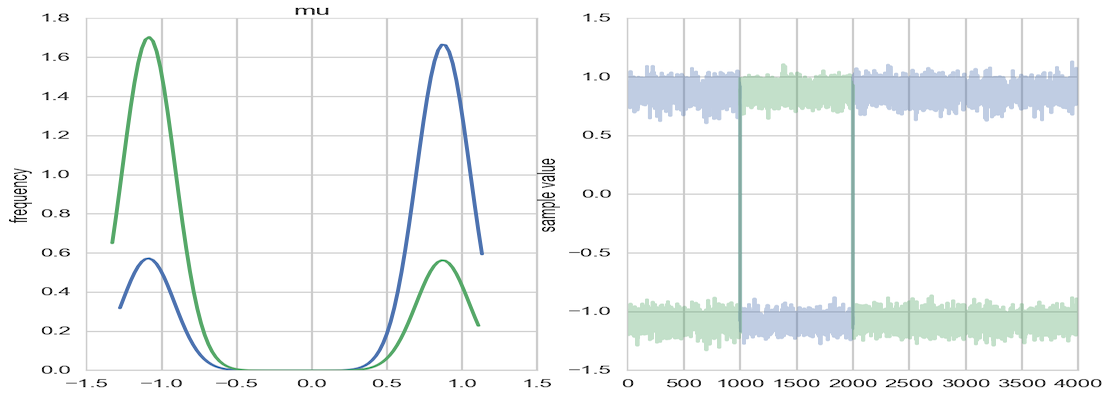
\includegraphics[width=\textwidth]{label_switching_example.png}
  \caption{Posterior samples and associated density plot from the posterior of a Gaussian mixture model with true parameters $\mu_1 = -1, \mu_2=1, \sigma_1=\sigma_2=0.75$. Left shows the density plot for the posterior of the mean parameters. Right shows the posterior sample trace. The label switches can be seen at samples 1000 and 2000 resulting in the multi-modal posterior on the left.}
  \label{fig:label_switching_example}
\end{figure}

\subsubsection{Algorithm Sketch}
Another possible solution for the identifiability problem is to provide labels for part of the data. This is termed semi-supervised learning and we incorporate this solution into our model. In the context of the CW domain, we can label observations as belonging to one regime or another. Let $S_{t, t+1,\ldots, t-1+K,t+K}$ be a consecutive set of $K$ state variables such that $S_t$ and $S_{t+K}$ have known value assignments (regime $m$ and regime $m+1$, respectively). The values for the state variables $S_{t+1,\ldots,t-1+K}$ are unknown. By Assumption 1, the switch between regimes $m$ and $m+1$ occurs at some $S_l$ where $t \leq l \leq t+K$. Therefore, the value of $S_l$ determines the values for all of the unknown states in this period as $S_t$ is assigned to regime $m$ for $t<l$ and it is assigned to regime $m+1$ for $t \geq l$.

We provide a sketch of this process in Algorithm~\ref{alg:constrained_alg}. \textbf{Step 1} initializes the $M$ supervised switch variables, one per regime. The labeled switch variables are spaced uniformly in time and are assigned to regimes in increasing order according to Assumption 1. This uniform method for initialization can be justified  by Assumption 2, in that  any set of regimes  that provides an interpretable model is sufficient. The number of expected  time steps in each period is $K=T/M$, and there are  $K-2$ unlabeled switch variables between each pair of  switch variables assigned to regimes.

\textbf{Step 2} performs MCMC sampling to approximate the posterior of the model. For the case when the value of the switch variable is known, the posterior of $X^{(m)}_t$ can be directly sampled by following the structure of a state space model. In the case where the switch variable is unknown, we have a marginalization problem over the two possible values of $S_t$. For the hidden Markov model (HMM) structure this can be efficiently computed with the forward algorithm~\citep{shumway2000time}. To formulate the HMM forward algorithm, we use the observation probabilities from the individual state space models in place of the emission probabilities of a standard HMM. Here, $\pi_{S_i}$ refers to the belief of the state of the switching variable given the evidence up to that point in time.

\textbf{Step 3} uses the regime specific parameters $\Phi^{(m)}$ to make a maximum a posteriori assignment of an observation to a regime using the Viterbi algorithm, thereby specifying the value of $S_t \forall t \in [1:T]$.

\LinesNotNumbered
\begin{algorithm}
\caption{Posterior inference algorithm}\label{alg:constrained_alg}
\textbf{Input: } $M$ (number of regimes), $\mathbf{Y}$ (vector of observations for $T$ time steps).\\
\nextnr
Initialization: Label one datapoint per regime, leaving $T - (M+1)$ unlabeled datapoints.\\
\nextnr
MCMC Inference: Draw samples for $X_{t}^{(m)}$ from the posterior distribution defined by the structured probability model:\\
	\For{$Y_t$ in $\mathbf{Y}$}{
		\eIf{$S_t=m$ is known}{sample from $P(X_{t}^{(m)}, \Phi^{(m)} \mid X_{t-1}, S_t=m, Y_t)$}
        {marginalize over $S_t$. Sample from  $\sum\limits_{i=m-1}^{m} \pi_{S_i}P(X_{t}^{(i)}, \Phi^{(i)} \mid X_{t-1}, S_t=i, Y_t)$}
	}
\nextnr
Posterior Inference: Use the posterior for regime parameters ($\Phi^{(m)}$) to run a Viterbi pass on the data $\mathbf{Y}$ to make a maximum likelihood assignment of the value of $S_t$ to regime $m$ (thereby learning the switching variables $S_t$).\\
\textbf{Output: } $S_t$ (assignments to regimes), $\Phi^{(m)}$ (regime specific posterior distributions).
\end{algorithm}

 Algorithm~\ref{alg:constrained_alg} can be computed on a SSSM where Assumptions 1 and 2 are appropriate. Such a model is shown in Figure~\ref{fig:updated_ssm_graphical_model}. The model depicts a subset of the time series with $K$ time steps from time $t$ to time $t+K$. There are two supervised labels at the boundaries of the subset with the variable $S_t$ assigned to regime $m$ and variable $S_{t+K}$ assigned to regime $m+1$. The unknown $K-2$ states in between are marginalized over such that the regime specific posteriors can still be approximated. This model is repeated for the $M-1$ switches in the data. The setup is flexible in that informative priors for the model noise and transition matrices can be specified (and related) as required by domain knowledge.

\begin{figure}
  \centering
  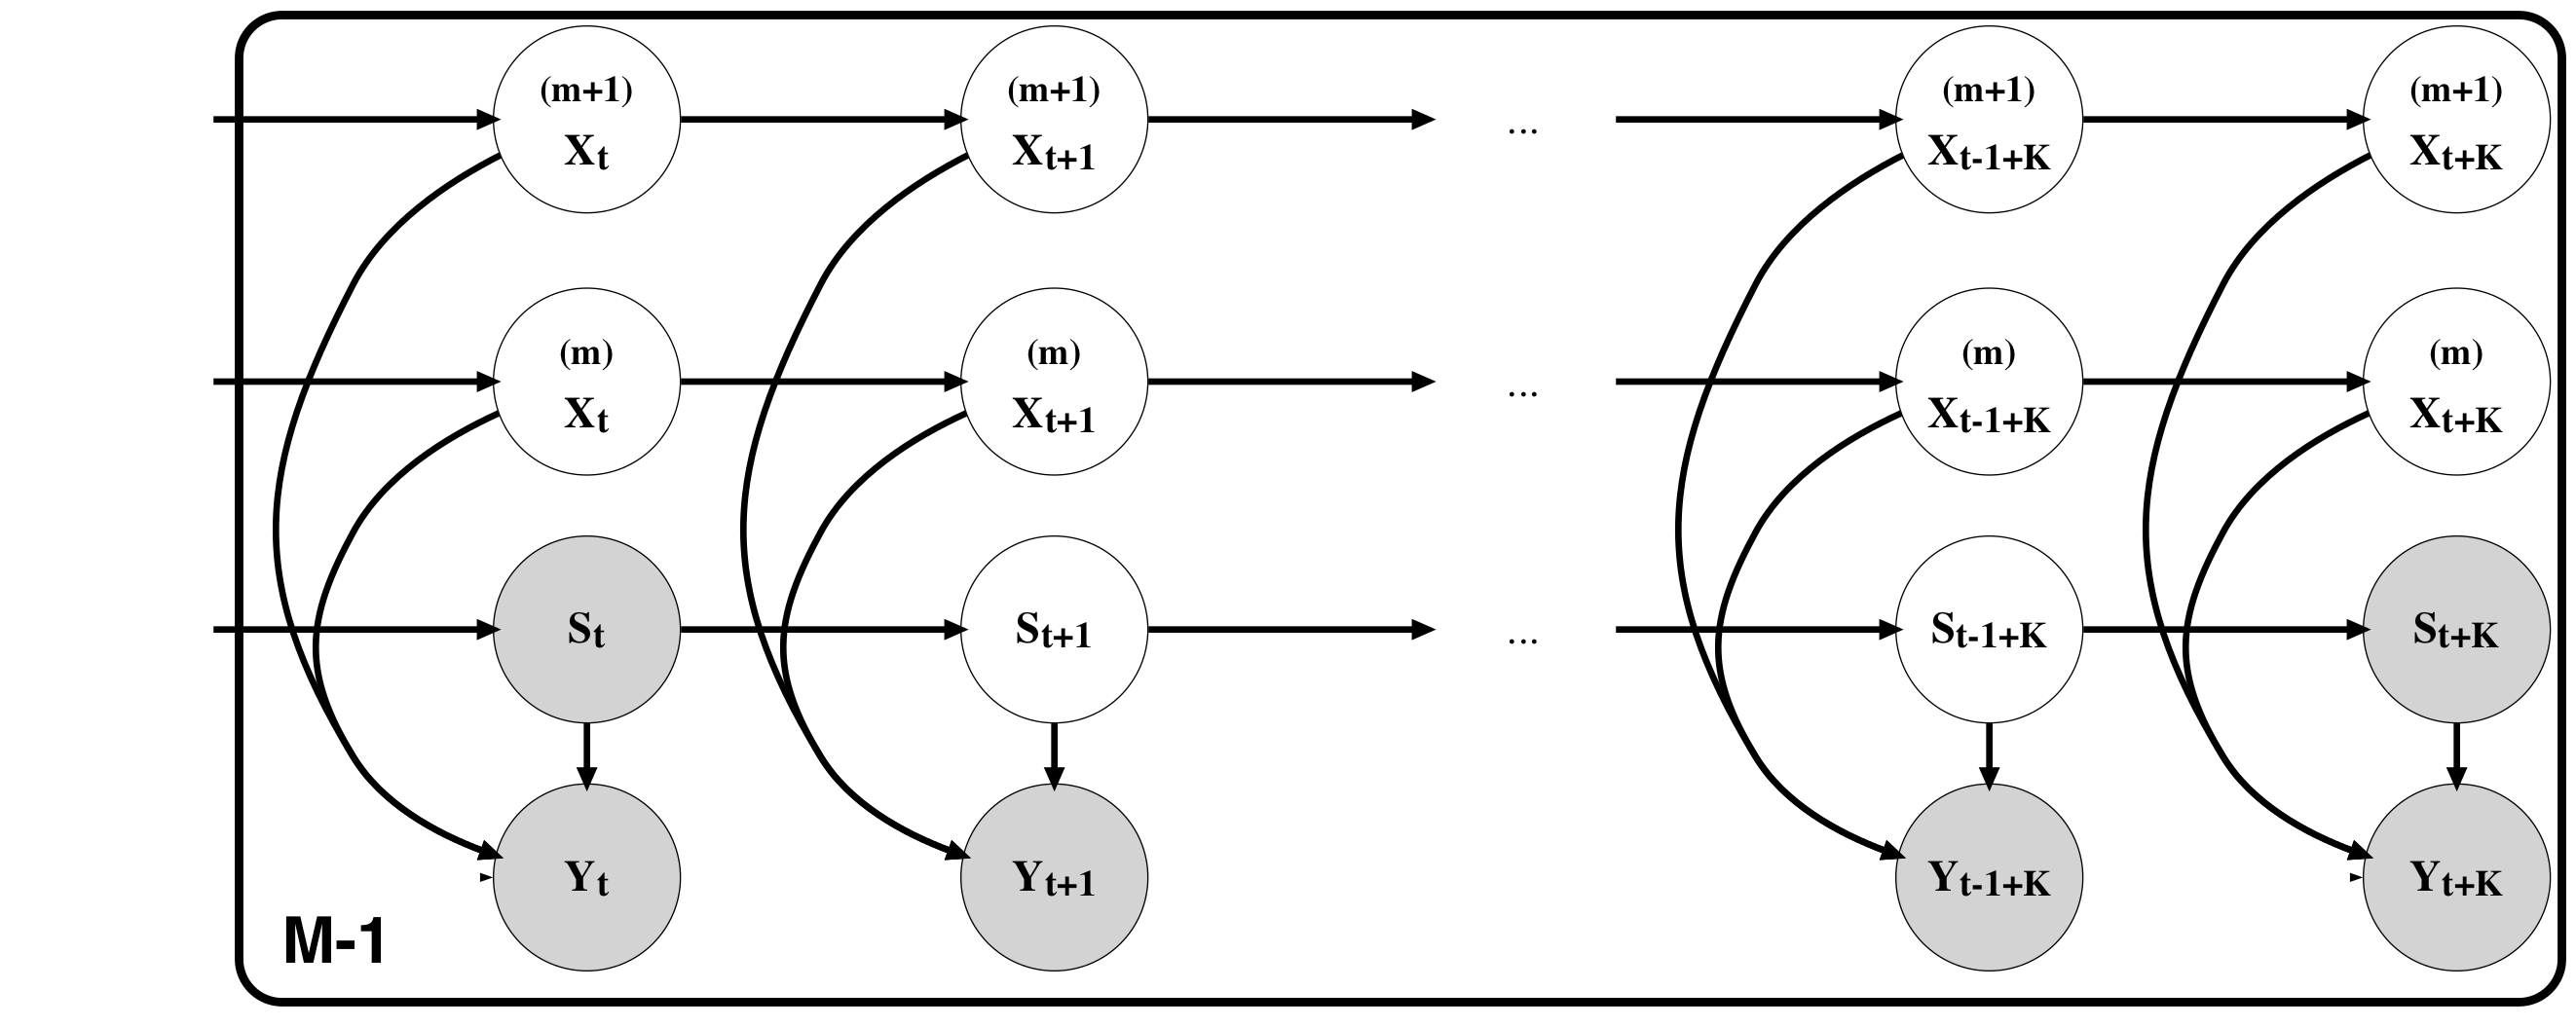
\includegraphics[width=\textwidth]{switching_ssm_constrained.png}
  \caption{Updated graphical model showing the semi-supervised switching labels, along with the choice of only two chains between two semi-supervised points. This representation is repeated $M-1$ times to describe the $M-1$ switches between the $M$ regimes. Note that the labeled switch variables at the boundaries ($S_t$ and $S_{t+K}$) are shared between successive regimes.}
  \label{fig:updated_ssm_graphical_model}
\end{figure}
